\chapter{The approximated regulator}
\label{app:approx}
\section{Why do we need an approximation?}

The problem is to compute the double integrals appearing in the threshold functions. 
In the case of the $O(n)$ model threshold functions are simple integrals, and the choice of the so-called $\theta$ regulator:
\begin{equation}
R_k(q) = (k^2 - q^2) \theta\left(1-\frac{q^2}{k^2}\right) 
\end{equation}
makes it possible to compute the integral explicitly. 
In the case of the Lifshitz model, we did not find a form of the regulator that made it possible to compute the double integral explicitly. 
However, we used the following multiplicative regulator based on the $\theta$ regulator:
\begin{equation}
R_t(q_\sslash^2, q_\perp^2) = R_\sslash(q_\sslash^2) r(q_\perp^2)
\end{equation}
with
\begin{equation}
r(q_\perp^2) = \left( 1 -\frac{q_\perp^2}{k^2} \right) \theta\left(1-\frac{q_\perp^2}{k^2} \right)
\end{equation}

All the integrals we will encounter are of the type
\begin{equation}
I_n(w) = v_m v_{d-m} \int_0^{\infty} dq_\sslash q_\sslash^{m-1} \int_0^{\infty} dq_\perp q_\perp^{(d-m)-1} \frac{\p{t} R_t(q_\sslash, q_\perp)}{\left[ a(q_\sslash^2) + Z_\perp q_\perp^2 + R_t + w \right]^n}
\end{equation}
This gives rise to integrals in the $\perp$ direction which are all of the type
\begin{equation}
J_{nD} = \int_0^{1} dq_\perp \frac{q_\perp^D}{\left[ a(q_\sslash^2) + Z_\perp q_\perp^2 + R_\sslash(q_\sslash^2) \left(1-\frac{q_\perp^2}{k^2} \right) \right]^n}
\end{equation}
The good thing is that these integrals can be expressed ``explicitly'' in terms of an hypergeometric function
\begin{equation}
J_{nD} = \frac{k^{D+1} \ _2F_1\left((1+D)/2,n;(3+D)/2;-\frac{b}{a}\right)}{(D+1)a^{n}}
\end{equation}
with
\begin{align}
a = a(q_\sslash^2) + R_\sslash + w \\
b = Z_\perp k^2 - R_\sslash(q_\sslash^2)
\end{align}

The ratio $a/b$ actually only depends on the dimensionless quantities $\bar{\rho_0}$ and $y_\sslash$. Dropping the bar on the dimensionless $\rho_0$, we define the function of dimensionless variables
\begin{equation}
h(D, n, y_\sslash, \rho_0) \define \ _2F_1\left((1+D)/2,n;(3+D)/2;-\frac{b}{a}\right)
\end{equation}

We could compute the integral in the $\perp$ direction, but we still need to compute the integral in the $\sslash$ direction. Sadly, the function $h$ depends on $y_\sslash$, which makes it impossible to compute analytically the integral. At this point we had the choice either to compute the integral numerically at the moment we solve the flow equations, or to try to find a good approximation that let us ``almost'' compute the integral analytically. We chose the second option because it facilitates the numerical integration of the flow equations, and of course also because the approximation we found is acceptable!

\section{The approximation}

\begin{figure}[htp]
\centering
\begin{subfigure}{.5\textwidth}
	\centering
	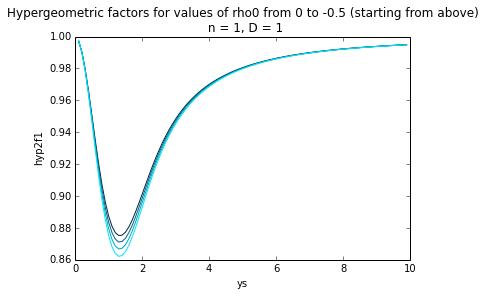
\includegraphics[width=.9\linewidth]{img/approx/hyp2f1.png}
	\caption{Plot of $h(D=1,n=1,y_\sslash,\rho)$ as a function of $y_\sslash$ for several values of $\rho_0$.}
	\label{fig:h}
	\end{subfigure}%
\begin{subfigure}{.5\textwidth}
	\centering
	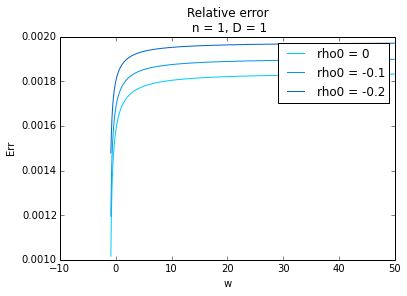
\includegraphics[width=.9\linewidth]{img/approx/relat_err.png}
	\caption{Relative error in $I_1(w)$ as a function of $w$.}
	\label{fig:I1}
\end{subfigure}
\caption{}
\label{fig:approx}
\end{figure}


We made the approximation $h \simeq 1$, which at first sight can seem rather brutal. As we are going to see, it can be quite well justified!

The approximation consist in replacing the curves appearing in fig. \eqref{fig:h} by the straight line $h = 1$. The greater $D$ and $n$ are, the deeper the ``well'' we see in the figure is deep. Therefore the worst case for doing the approximation is $n=1$ and $D=1$. In this case, we have plotted the function for several values of $\rho_0$, to make it clear that the greater $\rho_0$ is in module, the worse the approximation will be. From numerical computations (see the last section of the report for the details) we have seen that $\rho_0 \in [-0.2, 0]$. Therefore $\rho_0=-0.2$ is the worst case for us. 


To see how good our approximation is, we have computed numerically the integral $I_{n=1}$, with and without the approximation. The graph of the relative error as a function of the argument $w$ of the threshold function is shown in fig. \eqref{fig:I1}. In all our computations, $w$ is either $u'(\rho)$ (massless modes) or $u'(\rho) + 2 \rho u''(\rho)$ (massive mode). It can shown, invoking the convexity of the $\gam_t^{\text{Leg}}$ function, that these arguments can never be less than $-1$. This is why we focused on $w \in [-1, \infty]$.

We see that in the worst case the error is of approximately $0.2~\%$, which is good, given the precision we seek on the critical exponents.
With this approximation, all the computations can be done analytically, leading to flow equations we very easily solved numerically.